
%(BEGIN_QUESTION)
% Copyright 2007, Tony R. Kuphaldt, released under the Creative Commons Attribution License (v 1.0)
% This means you may do almost anything with this work of mine, so long as you give me proper credit

Shown here is the response of a proportional+integral controller to a step-change in process variable (with a constant setpoint).  Calculate the controller's proportional and integral constant settings, based on what you see in the graph.  Also, determine whether this controller is direct or reverse acting, and mark the features of the output plot corresponding to proportional action and to integral action.

$$\includegraphics[width=15.5cm]{i01601x01.eps}$$

The time scale on the chart is minutes:seconds, and the PI algorithm is as follows:

$$m = K_p \left( e + {1 \over \tau_i} \int e \> dt \right) + b$$

\noindent
Where,

$m$ = Controller output (manipulated variable)

$K_p$ = Gain

$e$ = Error signal (SP$-$PV or PV$-$SP)

$\tau_i$ = Integral time constant

$b$ = Bias

\vskip 10pt

\vskip 20pt \vbox{\hrule \hbox{\strut \vrule{} {\bf Suggestions for Socratic discussion} \vrule} \hrule}

\begin{itemize}
\item{} When analyzing the output trend of a PI controller, the definition of the reset time constant as being ``the number of minutes required to per repeat proportional action'' is most useful.  Identify the magnitude of proportional action in response to the PV step-change, and then explain how this value is helpful in identifying $\tau_i$.
\item{} Re-sketch what the output trend would look like if this controller's gain value ($K_p$) were doubled.
\item{} Re-sketch what the output trend would look like if this controller's integral time constant ($\tau_i$) were doubled.
\item{} Re-sketch what the output trend would look like if this controller's bias value ($b$) were increased.
\end{itemize}

\underbar{file i01601}
%(END_QUESTION)





%(BEGIN_ANSWER)

Controller action = {\it reverse}
 
\vskip 10pt

Gain constant = 0.5
 
\vskip 10pt

$\tau_i$ = 1 minute per repeat ($K_i$ = 1 repeat per minute)
 
%(END_ANSWER)





%(BEGIN_NOTES)

We know this controller's action is {\it reverse} because the output decreases as the process variable input (PV) increases.  Its gain is calculated by the ratio of the output step-change magnitude to the input step-change magnitude: in this case, a 5\% output step-change is caused by a 10\% input step-change, for a gain of 0.5.  We see that over a minute's period of time, the integral action causes the output to drift another 5\% (the trend shows a 10\% drift over 2 minutes), indicating an integral constant value of 1 repeat per minute.

%INDEX% Control, proportional + integral: graphing controller response

%(END_NOTES)


